\documentclass[10pt,a4paper]{ctexart}
\usepackage[margin=0.72in]{geometry}
\usepackage{graphicx}
\usepackage{enumitem}
\usepackage{xcolor}
\usepackage{array}
\usepackage{tabularx}
\usepackage{hyperref}
\pagestyle{empty}
\setlist[itemize]{leftmargin=1.5em, itemsep=0pt, topsep=1pt, partopsep=0pt}
\setlist[enumerate]{leftmargin=1.7em, itemsep=0pt, topsep=1pt, partopsep=0pt}
\definecolor{mainblue}{HTML}{1F4E79}
\definecolor{deepgray}{HTML}{333333}
\newcommand{\sectiontitle}[1]{\noindent{\large\bfseries\color{mainblue}#1}\vspace{0.2em}\hrule\vspace{0.35em}}
\linespread{1.1}
\begin{document}
\noindent
\begin{minipage}[t]{0.72\textwidth}
\vspace{0pt}
{\huge\bfseries\color{mainblue} 王世鑫} \\
\vspace{0.3em}
\renewcommand{\arraystretch}{1.1}
\begin{tabular}{@{}ll}
\textbf{出生年月：} 1995.04 & \textbf{籍贯：} 河南 \\
\textbf{毕业学校：} 中国人民大学 & \textbf{学历：} 博士 \\
\textbf{性别：} 男 & \textbf{电话：} 18810196936 \\
\textbf{邮箱：} wangshixin@ruc.edu.cn & \textbf{求职方向：} 数据科学 / 人工智能
\end{tabular}
\end{minipage}
\hfill
\begin{minipage}[t]{0.18\textwidth}
\vspace{0pt}
\centering
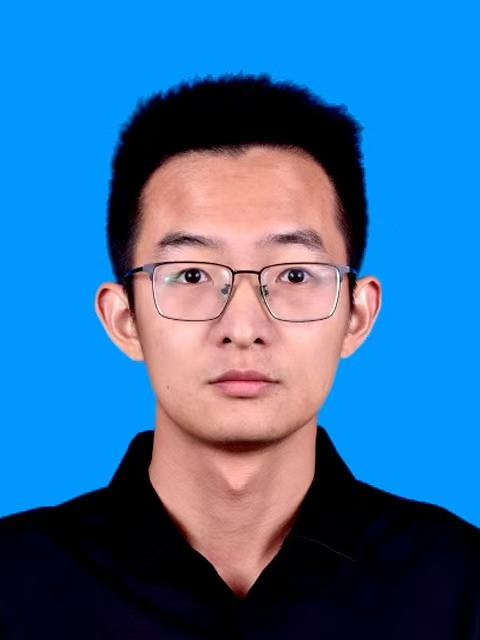
\includegraphics[width=2cm]{照片.jpg}
\end{minipage}
\vspace{0.6em}

\sectiontitle{求职意向}
\noindent
人工智能、大模型、信号处理、数据科学，长期关注前沿技术研究与工程落地，致力于利用数据驱动与智能算法提升产品能力与科研创新水平。

\sectiontitle{擅长技能}
\begin{itemize}
\item 熟悉数据科学、深度学习、强化学习模型方法；熟悉大模型算法
\item 熟练使用python，掌握linux环境，git版本控制等
\end{itemize}

\sectiontitle{学习经历}
\noindent
\textbf{博士} \quad 中国人民大学 \hfill 2020.09 -- 2026.12 \\
\textit{专业：} 概率论与数理统计 \\
\textit{研究方向：} 分布式光纤传感、信号处理与多目标轨迹跟踪 \\
\textit{研究成果：} 围绕光纤传感信号处理与多目标轨迹跟踪开展算法研究。
\vspace{0.3em}

\noindent
\textbf{硕士} \quad 中国科学院大学 \hfill 2016.09 -- 2019.06 \\
\textit{专业：} 运筹学与控制论 \\
\textit{研究方向：} 社交网络影响力最大化、图论与组合优化 \\
\textit{主要成果：} 基于图论与组合优化方法研究信息传播建模与关键种子节点选取。
\vspace{0.3em}
 
\noindent
\textbf{本科} \quad 上海大学 \hfill 2012.09 -- 2016.06 \\
\textit{专业：} 数学与应用数学 \\

\sectiontitle{实习经历}
\noindent
\textbf{神农智算} \quad \textit{智能穿戴与数字健康算法工程师实习} \hfill 2026.03 -- 2026.09 \\
\begin{itemize}
\item 面向数字健康场景从事智能穿戴感知数据处理与分析，设计算法提取生理信号特征，获得目标结果；
\item 参与数据采集、预处理、算法开发到实验验证的完整链路。
\end{itemize}

\sectiontitle{科研经历}
\noindent
\textbf{基于高速公路多模态复杂数据的深度学习模型研究} \hfill 2021.06 -- 2022.12 \\
\begin{itemize}
\item 视频目标检测与追踪：处理高速路视频数据，实现AI算法准确识别车辆目标，通过改进训练方法与数据集提升识别效果，解决自采数据集特有识别问题；
\item 点云目标检测：研究深度学习算法实现点云目标识别，处理Kitti、nuScenes等经典点云数据集，使用mmdetection3D框架测试模型检测效果；
\item 光纤数据分析与信息提取：研究光纤数据特点并提取关键信息，分别采用传统算法与深度学习方法完成数据去噪与关键点提取。
\end{itemize}

\sectiontitle{工作经历}
\noindent
\textbf{优策科技有限公司} \quad \textit{算法专员} \hfill 2019.07 -- 2020.02 \\
\begin{itemize}
\item 样本生成：利用生成式对抗网络(GAN)学习数据特征，对历史数据中缺失时间段的样本进行生成补全；
\item 旅客量预测：基于神经网络回归模型实现旅客量预测功能，结合决策树完成数据分类与标注。
\end{itemize}

\sectiontitle{发表文章}
\begin{enumerate}
\item \textbf{第一作者}. \textit{Leveraging a Repetitive Filtering Framework for Robust Pulse Stream Extraction in Distributed Optical Fiber Sensing Signals}. Photonics, 2026.
\item \textbf{第一作者}. \textit{Topology-Aware Multi-Object Tracking for Continuous Vehicle Trajectory Extraction Using Distributed Acoustic Sensing}.
\end{enumerate}

\end{document}
